\logg{Onsdag 02. Oktober}{10:00 til 14:00 (4 timer)}{
Møtte opp klokken 10:00 i dag. Kom tilbake til kontoret med møtet på at datamaskinen min er død. Dette er et problem ettersom gjenopprettingen av databasen ikke ble fullført. Heldigvis var mye av den relevante dataen gjenopprettet, noe som gjør at studenten bestemte seg for å ikke jobbe mer med det. \\

Dermed bestemte studenten seg for å fortsette å kode matematikken/logikken som skal brukes i applikasjonen. Her lagde studenten noen \textit{Issues} om hva som må bli gjort.

\begin{figure}[H]
\centering
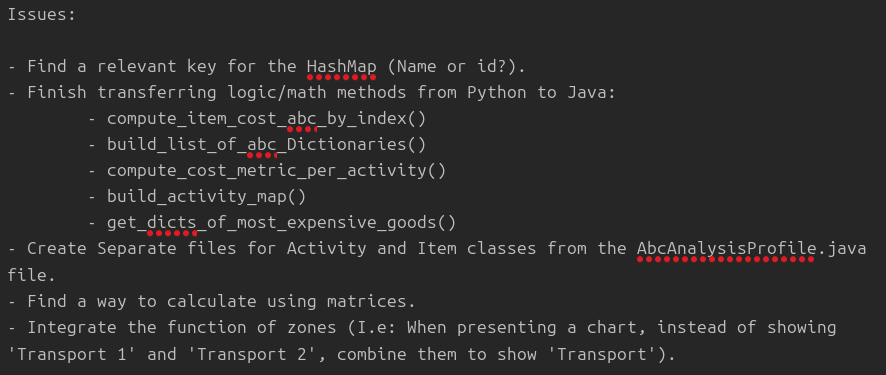
\includegraphics[width=1\linewidth]{ukentlige logger/images/uke 4/issues 02.10.png}
\caption{\label{fig:downloads}Issues fra Onsdag 02. Oktober.}
\end{figure}

Studenten Vegard Arnesen Mytting dro for å rekke en forelesing klokken 14:00.
}\\\\\\